% Terms and Definitions
%TODO maybe move stuff from chapter 1 in this chapter
\chapter{Metrics and Measurement Methods}

[tbd]

\begin{itemize}
	\item Last chapter...
	\item This chapter: In this chapter, I will cover measurement methods and discuss common performance metrics.
	\begin{itemize}
		\item This chapter should cover all relevant terms and definitions within web performance measurement
		\item How terms can be structured / taxonomy
		\item Ambiguity of definitions
	\end{itemize}
	\item In the next chapter...
\end{itemize}


- Technical Background:
	- Network
	- Front End: Navigation and CRP
	
- Metrics

- Measuring Methods



% TODO
% IF possible use more cool tables


% ---------------------------------------------------------------------------------------------------
% ---------------------------------------------------------------------------------------------------


%TODO find better title
\section{How Websites are being loaded}

% [Introduction]
- Brief technical introduction
- It is important to understand how things work, because Metrics and also how to measure them are derived from those processes

In order to understand web performance metrics and the methods to measure them, it is crucial to have a basic understanding of the technical aspect of loading a website into a browser.
This process includes establishing a connection between a client and a server, which will be discussed in section X, and the task of the browser to transform the received data from the server into a readable ready-to-use website, which will be discussed in section X.
Always with performance in mind.

% [3 Entities: FE, BE, Network]
It is possible to divide the website loading process into three entities which play a role.
In his code talk 2016, Witt identifies three main areas or bottlenecks where bad performance is being produced: In the Frontend, the Backend, and on the network layer.  % cite 2016 Witt or just say this ??
The Front End is everyhting the user sees on the screen, client, UI, browser, sends requests to a back end, etc.
The Back End is the logic, servier, also data base, handles requests and sends responses to a front end
Network is what connects clients and servers, FE and BE, infrastructure element composed of routers, cables, wireless connections etc.


- BE is not discussed (server time, data base, etc.)
- Section X is about Network
- Section X is about Front end: how browser works, crp, 
- How to optimise websites is not part of this thesis

In this section, i will also say which metrics are describing the underlying process.
So this section links directly to the metrics section.
But all metrics are collected in the metrics section.



% --------------------------------------------------------------------------------------------
% --------------------------------------------------------------------------------------------


%TODO choose title. Maybe "Establishment of Connection?"
\subsection{The Network Realm}

Starting from hardware, ISP, routers, switches etc and the cables connecting them is part of the network.
But also communication protocols such as the Internet protocol suite.

Regarding performance, latency and bandwidth come into mind, and we will see that latency has a bigger impact on performance than bandwidth in section X.

After discussing this issue, i will continue by describing the process or navigation steps which happen once the user enters a URL into the browser, up until he sees pixels on his screen and can use the website.


% --------------------------------------------------------------------------------------------


\subsubsection{Latency and Bandwidth}

There are two important attributes when discussing network performance: Latency and Bandwidth.
The important thing to say here is that Latency is bottleneck for performance, and not bandwidth.


% [Bandwidth]

Bandwidth is the "maximum throughput of a logical or physical communication path". %cite 2013 Grigorik
In other words, bandwidth describes the amount of data which can be sent in parallel from one node in a network to another. 

Physical communication paths are most likely cables such as metal wires or fiber-optic cables, where fiber-optic cables have less signal loss, and lower lifetime maintenance costs.
With methods such as wavelength-division multiplexing (WDM), it is possible to transmit up to 70 Tbit/s over a fiber-optic connection.  %cite 2013 Grigorik

This high technology stuff is only used in the backbone infrastructure, e.g. for connecting Europe with America.
For the end user, bandwidth is much lower, and the average was in late 2015 just 5.1 Mbps %cite 2013 Grigorik

A high bandwidth is useful for bulk or large data transfer such as streaming of video or audio.
But for loading a website,or any browser activity that depends on many requests that fetch data from many different locations around the globe, the performance bottleneck is latency. % cite 2013 Grigorik


% [Latency]

Latency is "the time from the source sending a packet to the destination receiving it".  % cite 2013 Grigorik

Latency is measured in seconds and can be the time spent for one-way, or more common, how long it takes for the transmitted data package for the round-trip time (RTT), from source to destination and back.
In other words, latency "describes the amount of delay on a network or Internet connection". % cite https://developer.mozilla.org/en-US/docs/Web/Performance/Understanding_latency

For the very first request when establishing a connection, latency is longer due to protocols such as DNS lookup, TCP and TLS handshakes.
Those will be discussed in section X. % cite https://developer.mozilla.org/en-US/docs/Web/Performance/Understanding_latency


% [Experiment]

To get an idea about how the two aspects, bandwidth and latency, impact web performance,  Mike Belshe launched a study. % cite https://docs.google.com/a/chromium.org/viewer?a=v&pid=sites&srcid=Y2hyb21pdW0ub3JnfGRldnxneDoxMzcyOWI1N2I4YzI3NzE2
Once setup has a fixed latency and bandwidth is variable, and vice versa.
He and compared the performance of the two experiments using the Page Load Time metric. (cf. X for this metric)


\begin{figure}[h!]
\begin{center}
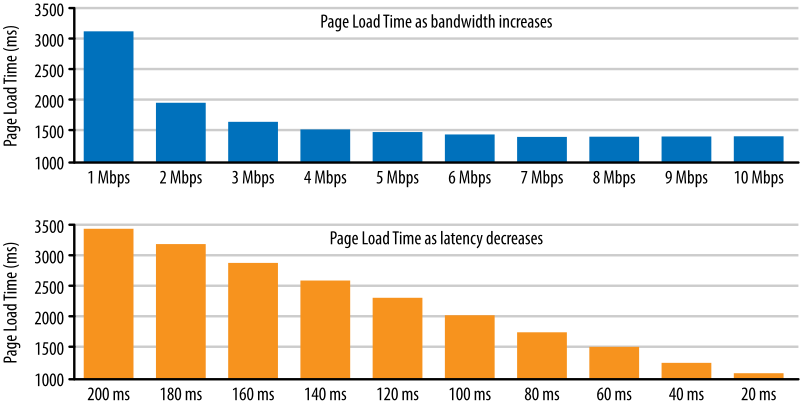
\includegraphics[width=0.8\textwidth]{latency.png}
\caption{Latency vs Bandwidth}
\label{img:latency}
\end{center}
\end{figure}


We can see that the impact of bandwidth is trivial: if the available bandwidth is doubled, e.g. from 5 to 10 Mbps, there is no change in performance load time.
For Latency on the other hand, the picture is different: If the latency can be decreased by half, e.g. from 120 ms to 60 ms, the page load time also sinkt um die hälfte.

Or as Belshe states it, "[reducing] cross-atlantic RTTs from 150ms to 100ms [...] would have a larger effect on the speed of the internet than increasing a user's bandwidth from 3.9Mbps to 10Mbps or even 1Gbps." % cite https://docs.google.com/a/chromium.org/viewer?a=v&pid=sites&srcid=Y2hyb21pdW0ub3JnfGRldnxneDoxMzcyOWI1N2I4YzI3NzE2

This obersvations can be explained with the many short, small connections and requests are made when browsing websites and the contrary underlying structure of the communication protocols, which are "optimized for long-lived connections and bulk data transfers. " %cite 2013 Grigorik ch 10

But just simply decreasing the latency is not straightforward: The speed of data transfer is already at a 2/3 of light, but the physical constraint is the limiting factor, e.g. there is a minimum distance between London and New York which can not be further "optimized". % cite 2013 Grigorik Ch 1


% [Mobile]

Another aspect of latency is that for wireless connections and therefore mobile devices, latency is even higher, "making networking optimization a critical priority for the mobile web." % cite 2013 Grigork Ch 1

This is due to the infrastructure of mobile nets, latency is high for mobile users. cf.  Why are mobile latencies so high? in Grigorik % cite https://www.igvita.com/slides/2013/fluent-perfcourse.pdf


% [Transition]

As latency is a important factor, what happens on the front end is still important.
And again for this thesis metrics measuring performance in the front end are the focus.

Before i will discuss what happens in the browser once the website data arrived, i will briefly describe the preceding steps of establishing a connection between the browser (client) and the server.



%TODO add this ?

% Use other techniques such as CDNs, caching, pre-fetching, etc % 2013 Grigorik
% CDN: Help against this issue. Put stuff close to client % 2013 Grigorik

% Some direct implications for performance measurement ?
% Understanding Latency https://developer.mozilla.org/en-US/docs/Web/Performance/Understanding_latency
% Network throttling: Emulate download speed, upload speed, and minimum latency



% --------------------------------------------------------------------------------------------



\subsubsection{Navigation Process}

I will explain briefly the general navigation process: It begins when the user is submitting a URL in the browser and ends when he received website data.

The main steps can be divided into networking, that is, establishing a connection with DNS etc., backend processing, e.g. data base queries etc., and the rendering in the front end, as seen in image X.
The last part of this process is when browser receives finally the HTML / Document. 
How the browser transfers the HTML into an interactive website is part of the next section.


"To start, it is important to recognize that every HTTP request is composed of a number of separate stages (Figure 10-3): DNS resolution, TCP connection handshake, TLS negotiation (if required), dispatch of the HTTP request, followed by content download." % cite Grigorik 2013


\begin{figure}[h!]
\begin{center}
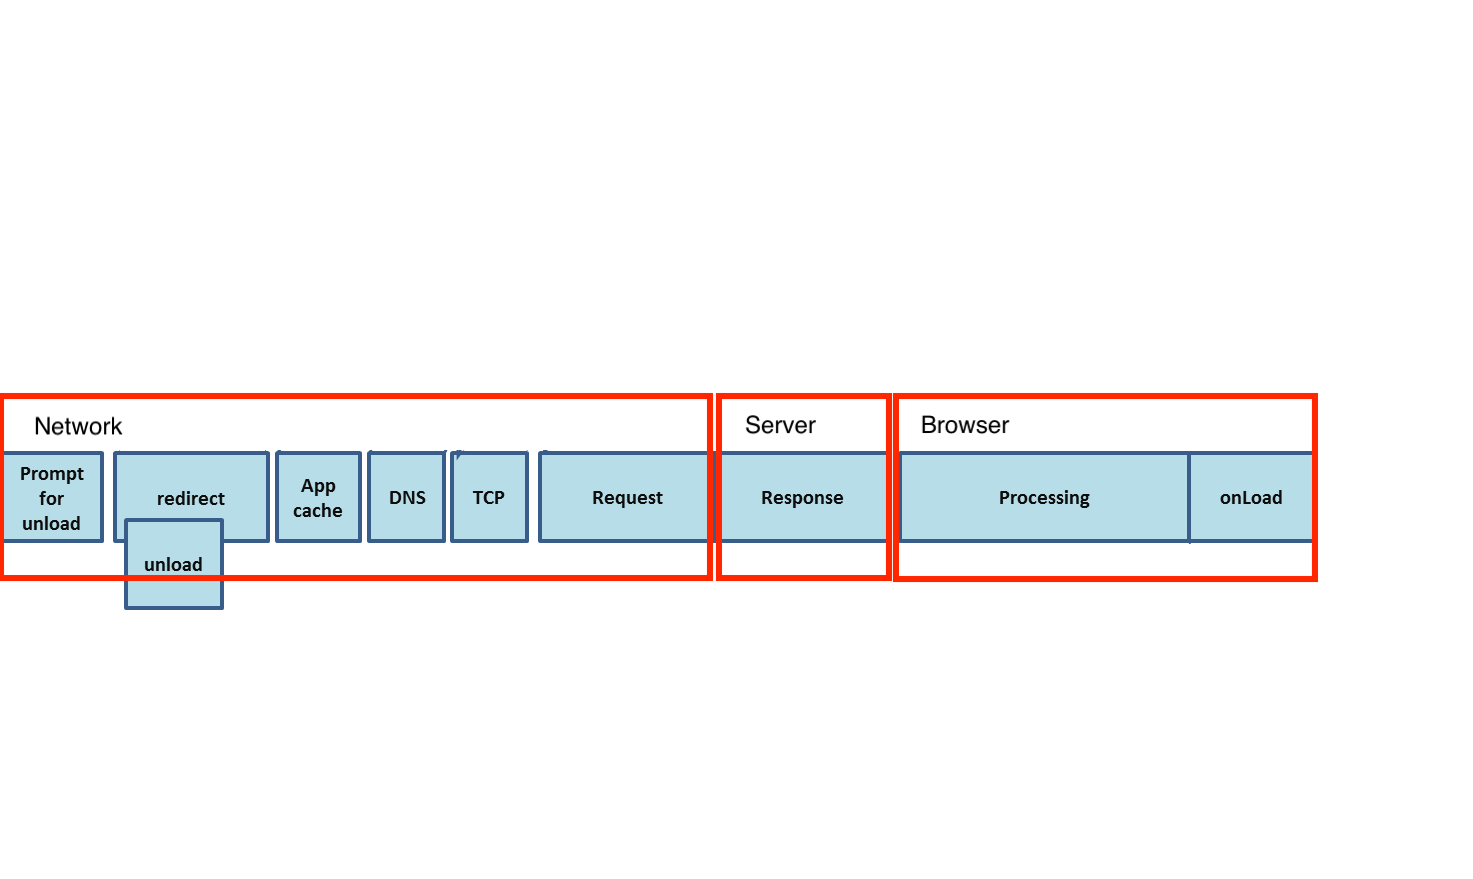
\includegraphics[width=0.8\textwidth]{timing_overview.png}
\caption{Timing Overview}
\label{img:timing_overview}
\end{center}
\end{figure}
%TODO change image: remove network and BE boxes? remove white space around image


%TODO add this ?
% Understanding Latency https://developer.mozilla.org/en-US/docs/Web/Performance/Understanding_latency
%Network Timings:
%- Blocked: When a request is in queue
%- Blocking happens when there are too many simultaneous connections to single server over HTTP



% ----------------------------------


\paragraph{DNS Lookup}

When the requested resource can not be loaded from the browsers cache, the first step to establish a connection is a DNS Lookup (or DNS Resolution).

This step is about translate URL to IP address.
Must be done for each unknown URL, e.g. when linked images within a website are from different server, for each unique URL DNS Lookup has to be done.
The mapping of URL to IP can be cached by browser, which makes repeated views faster. % cite https://developer.mozilla.org/en-US/docs/Web/Performance/How_browsers_work

Avg. time is 20 and 120 ms % https://www.keycdn.com/support/reduce-dns-lookups
Can be considered a performance metric, see section X.


% ----------------------------------


\paragraph{TCP Handshake}

Once a connection between a client and a server is established, the TCP 3-way-Handshake comes into play.

The goal of TCP is to establish a reliable connection within an unreliable network.
TCP  "guaranteed that all bytes sent will be identical with bytes received and that they will arrive in the same order to the client. " %cite 2013 Grigorik
Regarding performance, the handshake adds two more round trips, which is bad for performance as we have seen because of latency.

Many algorithms and techniques to get optimal data transfer and also avoid congestion are existing, such as Slow-Start.
Slow-Start is an algorithm that determines the maximum bandwidth that can be used by gradually increasing the amount of data sent.
Slow start prevents that the full capacity of the network is being used from the beginning, which in performance terms adds again more round trips and latency. %cite 2013 Grigorik


%TODO once i know which metric add it here
A performance metric reflecting the time spent for establishing a TCP connection is X, see section X.
For a detailed discussion cf "Building Blocks of TCP" in 2013 Grigorik % cite https://hpbn.co/building-blocks-of-tcp/


% ----------------------------------


\paragraph{TLS Negotiation}

TLS is another protocol which has the goal to establish a secure connection in terms of data encryption.
Data transmitted over the network has to be encrypted so that aussenstehende can not read or manipulate the data.
For encryption,  a cipher to be used needs to be established, which will be shared between client and server during the TLS Negotiation. % cite https://developer.mozilla.org/en-US/docs/Web/Performance/How_browsers_work

TLS again adds more round trips which is bad for performance.

%TODO once i know which metric add it here
A performance metric reflecting the time spent for a TLS negotiating is blabla in section X.

for a detailed discussion see Transport Layer Security (TLS) in 2013 Grigorik % https://hpbn.co/transport-layer-security-tls/


% ----------------------------------


\paragraph{HTTP Request and Response}

Now that a secure connection is established, the client fetches the first resources via HTTP GET request.
Most often, the server will respond by sending back the index.html file, which then can be used by the browser to build the website. % cite https://developer.mozilla.org/en-US/docs/Web/Performance/How_browsers_work

The time when this first response containing the first byte for building the web site is reflected in the metric TTFB which is discussed in section X.


% [Connection vs Request]

Usually, many more resources are requested by the browser to complete the build of the web site.
As of today, the median value is about 70 requests per web site. % footnote https://httparchive.org/reports/state-of-the-web#reqTotal

A request is not the same as a connection.
Once the connection is established via the above described procedures such as DNS lookup, TCP and TLS handshakes, multiple requests can be transmitted over the same connection.
Usually, the number of requests is much higher than the number of connections to load a website, as the browser persist connections, keep them open for multiple requests.
Median connections for a web site today is about 13. % footnoe https://httparchive.org/reports/state-of-the-web#tcp
Modern browsers like Chrome enable up to six open connections in parallel. % cite 2014 Hogan



% [Transition to CRP]

At this point, the browser has received the first data about the web site and he can start with rendering the page.
How this exactly happens, is explained in the next section.




% --------------------------------------------------------------------------------------------
% --------------------------------------------------------------------------------------------



\subsection{Front End: Critical Rendering Path}

This section explains what happens after the first bytes of the web sites arrived in the browser.
The following processes are typically subsumed under the term \textit{Critical Rendering Path} (CRP).
The CRP is the last part of the navigation process as seen in image X.


% [Critical]

The CRP is the minimum steps that the browser has to take from the moment it receives the first byte of HTML to the moment that it renders pixels on the screen for the first time.

The rendering is critical as it is the very first render, the first visible content the user will see on the screen.
The resources that are needed for the first render of the page delay the first render of the page are considered to be critical.
Without the critical resources, the browser can not display content on the screen.
An example of a critical resource is the first HTML file the browser receives, as without it, nothing is visible on the screen.
Non-critical resources on the other hand will not stop the browser from displaying the first content on the screen. % cite https://blog.logrocket.com/how-css-works-parsing-painting-css-in-the-critical-rendering-path-b3ee290762d3/


% https://gtmetrix.com/blog/how-to-eliminate-render-blocking-resources/
%- Non-critical resources are those that provide contributions to secondary/tertiary functionality or styling for the content on your page, e.g., a calendar widget on the sidebar below-the-fold.


% https://blog.logrocket.com/how-css-works-parsing-painting-css-in-the-critical-rendering-path-b3ee290762d3/
%- Any CSS that is not necessary for the first load can be considered “non-critical”



% [CRP Steps]

There are a sequence of steps the browser goes through to render the page.
The basic idea is to convert HTML, CSS and JS to actual pixels on the screen.

Image X visualizes the flow of the CRP:
Once the HTML is received, the browser starts with parsing the HTML and translate it into the DOM.
The content of the CSS files will be parsed to the CSSOM.
JavaScript needs to be fetched and executed.
Once DOM and CSSOM are available, the Render Tree is being created.
When the Render Tree is available, Layout is happening.
Finally, pixels can be printed on the screen.
% cite https://developer.mozilla.org/en-US/docs/Web/Performance/Critical_rendering_path

In the following, the individual steps will be discussed in more detail.


\begin{figure}[h!]
\begin{center}
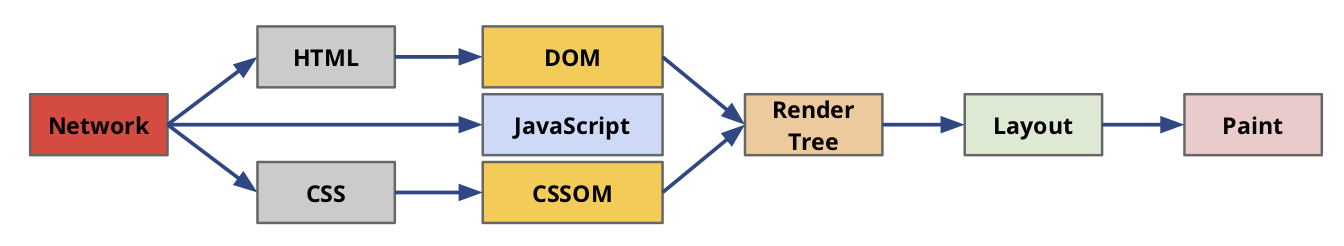
\includegraphics[width=0.7\textwidth]{crp.png}
\caption{Critical Rendering Path}
\label{img:crp}
\end{center}
\end{figure}




% [Single Thread]
%TODO do i need this ?
% How Browsers Work https://developer.mozilla.org/en-US/docs/Web/Performance/How_browsers_work
%- This is somewhat the bottleneck or the technical state of the browser
%- Browser is single threaded
%- Still: Enable smooth interaction: scrolling, responsive to touch, etc.
%- Render time is key
%- Goal: Main thread can complete all the work and still is available to handle user interaction
%-> Improvement: Understand single thread concept of browser and minimize main threads responsibilities
%-> Should lead to: rendering is fast and smooth and responses to interactions are immediate



% ------------------------------------------------------------


\paragraph{From HTML to DOM}

% [Introduction, Standard]

Once the browser received the first bytes of the HTML file, it starts to parse it into the \textit{Document Object Model} (DOM).
The DOM construction is the first step the browser performs when receiving data.
The DOM is a tree structure and internal representation of the HTML for the browser. % cite https://developer.mozilla.org/en-US/docs/Web/Performance/How_browsers_work
The general parsing process consists of translating from bytes to characters, to tokens, to nodes and finally to the object model.% cite https://developers.google.com/web/fundamentals/performance/critical-rendering-path/constructing-the-object-model
The specification of the DOM is maintained by the WHATWG living standard. % footnote https://dom.spec.whatwg.org/

% The Parsing of the HTML into the DOM is defined in the HTML standard % footnote https://html.spec.whatwg.org/multipage/parsing.html#parsing


% [Render Blocking]

The DOM tree contains information about the content of the document, but not its style.
The styling is defined in the CSS.
Once HTML and CSS are transmitted and processed by the browser, the \textit{Render Tree} can be created, which reflects the actual information and its styling the browser can display.
Within this context, it is possible to categorise resources into render blocking and non-render blocking.
A render blocking resource is a resource that prevents the browser from rendering content to the screen.
HTML and CSS are render blocking resources, as the parsing process of those files blocks the browser of displaying the page to the screen.% cite https://developers.google.com/web/fundamentals/performance/critical-rendering-path/render-blocking-css

% CSS parsing and render tree construction will be discussed below.


% [Incrementally]

As soon as the first data packages of HTML arrive at the browser, the parsing process starts. %cite How Browsers Work https://developer.mozilla.org/en-US/docs/Web/Performance/How_browsers_work
The DOM is created incrementally,  this means that the browser can begin to process the HTML before all of its content is transmitted over the network.


% [Resources]

Usually, within the HTML, external resources are linked which are necessary for the website to be complete, such as CSS or JavaScript.
While parsing the HTML incrementally, eventually a reference to such an external resource will be encountered.
How the external resources CSS and JavaScript are being handled by the browser is discussed below.


%TODO add this?

% How Browsers Work https://developer.mozilla.org/en-US/docs/Web/Performance/How_browsers_work
%- DOM is also exposed, and can be manipulated through various APIs in JavaScript 
%Optimisation: Preload scanner:
%- This process occupies main thread while browser is building DOM Tree
%- parse through the content available and request high priority resources like CSS, JavaScript, and web fonts.
%- will retrieve resources in the background so that by the time the main HTML parser reaches requested assets, they may possibly already be in flight, or have been downloaded




% ------------------------------------------------------------


\paragraph{From CSS to CSSOM}


% [Introduction]

The CSS resource contains all information about the styling of the page.
As with the HTML,CSS is converted from bytes to characters, to tokens, to nodes, and finally to the \textit{CSS Object Model} (CSSOM). % cite https://developers.google.com/web/fundamentals/performance/critical-rendering-path/constructing-the-object-model
CSSOM construction is usually very fast . % cite % How Browsers Work https://developer.mozilla.org/en-US/docs/Web/Performance/How_browsers_work
CSSOM is standardized here % footnote https://drafts.csswg.org/cssom/

% The DOM and and CSSOM are separated structures and not yet connected.
% The Render Tree reflects the combination of the two models and will be discussed below.
% Creation of CSSOM happens after DOM is completed. % https://developer.mozilla.org/en-US/docs/Web/Performance/Critical_rendering_path



% [Cascading, Not incrementally]

As opposed to the HTML parsing process, CSS can not be translated to the CSSOM incrementally.
Cause it the cascading nature of style sheets, which has the potential that the styling rules defined at the top of the file may be overridden by rules defined at the very end of the CSS file.
A partial CSSOM is therefore not possible.
Hence the browser needs the entire CSS file before he can create the CSSOM.
%cite  https://developer.mozilla.org/en-US/docs/Web/Performance/Critical_rendering_path


% [Not Parser Blocking]

As soon as the parser encounters a reference to an external style sheet such as

%TODO add caption={} ?
\begin{lstlisting}[language=html, numbers=none]
<link rel="stylesheet" href="styles.css">
\end{lstlisting}

it requests the resource and continues with parsing the HTML.
CSS is not a parser blocking resource.
When the CSS arrived at the browser, the CSSOM construction starts.
%cite  https://blog.logrocket.com/how-browser-rendering-works-behind-the-scenes-6782b0e8fb10/


%TODO add FOUC ?

% https://blog.logrocket.com/how-css-works-parsing-painting-css-in-the-critical-rendering-path-b3ee290762d3/
% - If it just went ahead and rendered to pixels without waiting for the CSSOM we’d see a flash of unstyled content (ugly!) for a moment while the CSSOM was parsing.



% [Render Blocking]

While CSSOM creation is not parser blocking, it is render blocking.
The browser blocks the page rendering until it received and parsed all of the CSS.
Rendering content to the screen is only possible when CSSOM and therefore CSS is available. % cite https://developers.google.com/web/fundamentals/performance/critical-rendering-path/render-blocking-css


% [When finished]

Once the DOM and CSSOM are created, they can be merged together into the render tree, which will be layout and painted to the screen.
Before I describe this process, I will discuss how JavaScript is being handled.


% [Optimization]

%TODO add this: optimization
%- You want to get CSS down to the user as quick as possible:
	%- Inlining styles
	%- Load not needed styles later
%- Optimization: use media queries
%- Better to add styles in single file
%- FOUC: Flash of Unstyled Content: If unstyled content is visible on the screen


% https://developers.google.com/web/fundamentals/performance/critical-rendering-path/render-blocking-css
%Media types and media queries allow us to mark some CSS resources as non-render blocking.


%TODO add this? Lighthouse what is render blocking https://web.dev/render-blocking-resources/
%Lighthouse flags resources as render blocking when:
%A <link rel="stylesheet"> tag that:
%Does not have a disabled attribute. When this attribute is present, the browser does not download the stylesheet.
%Does not have a media attribute that matches the user's device.





% ------------------------------------------------------------



\paragraph{What happens with JavaScript}


% [Introduction, Parser and Render Blocking]

JavaScript (JS) resources add functionality and interactivity to a web site.
When the browser encounters a script tag such as

%TODO add caption={} ?
\begin{lstlisting}[language=html, numbers=none]
<script src="myScript.js"></script>
\end{lstlisting}

it will stop its current task of parsing, fetch immediately the resource and execute its content, and only then proceed with the creation of the DOM. % cite % Grigorik Conference Talk https://www.youtube.com/watch?v=PkOBnYxqj3k&ab_channel=IlyaGrigorik
See image X.

JS can manipulate and query the DOM tree and directly change the HTML file.
As the HTML file is the input stream for the parser,  the parser stops until the JS is downloaded and executed. % cite https://developer.mozilla.org/en-US/docs/Web/Performance/Critical_rendering_path
Hence JS is parser blocking.
JS fetching and execution stops the parsing of the HTML and the construction of the DOM.
Only after the script finished execution, HTML parsing will continue.

Implicitly, because JS execution blocks DOM creation, and HTML processing itself is render blocking, JS is also render blocking. % cite Grigorik Conference Talk https://www.youtube.com/watch?v=PkOBnYxqj3k&ab_channel=IlyaGrigorik


The behaviour is the same for an external references JS file and a script directly added within in the HTML.


%TODO add this?

% This means that excessive scripts can be a significant bottleneck % How Browsers Work https://developer.mozilla.org/en-US/docs/Web/Performance/How_browsers_work

% https://blog.logrocket.com/how-browser-rendering-works-behind-the-scenes-6782b0e8fb10/
% - If the network is slow, and it takes thousands of milliseconds to fetch app.js, the DOM construction will be halted for the thousands of milliseconds as well

% https://blog.logrocket.com/5-tricks-to-eliminate-render-blocking-resources/
%- You can remove them from the critical rendering path by placing the <script> tags right before the closing </body> tag instead of the <head> section.
%-In this case, they only begin to download after the entire HTML has been downloaded.

% https://developer.mozilla.org/en-US/docs/Web/Performance/How_browsers_work
%- Though the browser's preload scanner hastens this process.


% [Blocked by CSS]

As JS can also manipulate the styling of the page, its execution is blocked until the CSSOM is available.
This means that the execution of the JS is on hold until the CSSOM is ready.
To summarize, while JS blocks the parsing of the HTML to the DOM, JS execution itself is blocked by the creation of the CSSOM.
CSSOM blocks JS, and JS blocks DOM construction. %cite 2013 Grigorik ch 10

Several attributes on the script tag can change the behaviour of the browser.
\textit{Async} and \textit{defer} are options to counter the blocking nature of the script tag.
They will be discussed now.\\



% [async attribute]

With the async (asynchronous) attribute, the browser downloads the JS in the background while continuing with the parsing of the HTML.
The parsing is not blocked and the browser can continue with his task. 
As soon as the JS is downloaded and available,  it is parser blocking: the browser stops the parsing and executes the JS.%cite https://developer.mozilla.org/en-US/docs/Web/HTML/Element/script

The order of all the async scripts within the document is not maintained any more.
Whenever a script is downloaded and available, it will be executed.
It does not matter if an async script was included at the top or bottom of the HTML document. % cite https://blog.logrocket.com/5-tricks-to-eliminate-render-blocking-resources/



% https://blog.logrocket.com/5-tricks-to-eliminate-render-blocking-resources/
%- The async attribute is recommended for independent third-party scripts, such as ads, trackers, and analytics scripts. For example, Google Analytics recommends adding the async attribute to support asynchronous loading in modern browsers.


% [defer attribute]

Like with async, scripts with the defer attribute enable the browser to download the script in parallel while continuing with the parsing of the HTML.
Contrary to async, defer scripts will only be executed after the parsing of the page is complete and the DOM tree is fully constructed,  and the order of the scripts will be maintained.  %cite  https://blog.logrocket.com/5-tricks-to-eliminate-render-blocking-resources/


%TODO add this nice graphic and cut out last rows https://html.spec.whatwg.org/multipage/scripting.html#attr-script-async
\begin{figure}[h!]
\begin{center}
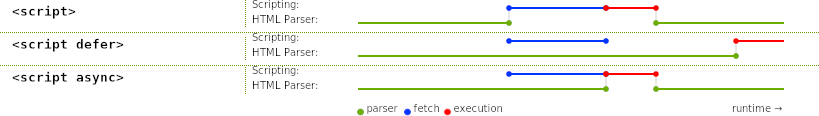
\includegraphics[width=0.8\textwidth]{scripts.png}
\caption{Scripts}
\label{img:latency}
\end{center}
\end{figure}


The async and defer attributes not applicable on inline scripts.
From the standard, "scripts may specify defer or async, but must not specify either unless the src attribute is present. " % \footnote https://html.spec.whatwg.org/multipage/scripting.html#attr-script-async
As inline scripts do not contain a src attribute, as the source of the script is within the script tags, the async and defer attributes are not applicable.


% https://blog.logrocket.com/5-tricks-to-eliminate-render-blocking-resources/
%- The defer attribute is recommended for scripts that need the DOM, but you want to begin to download them before the document loads, without making them a render blocking resource.
%- You should also use defer rather than async if the document order is important — for instance, when consecutive scripts depend on each other.



% [Transition]





% [More stuff]

%TODO add this? preload scanner
% https://developer.mozilla.org/en-US/docs/Web/Performance/How_browsers_work
%- Though the browser's preload scanner hastens this process.

% Grigorik Conference Talk https://www.youtube.com/watch?v=PkOBnYxqj3k&ab_channel=IlyaGrigorik
% And slides https://www.igvita.com/slides/2013/fluent-perfcourse.pdf
%- Asynchronous pattern:
	%- Not the same as async/defer tag
	%- Will fetch JS asynchronously
	%- Uses IIFE which creates a new script tag in the HTML with attribute async
	%see chapter X how Google Analytics is doing this.


%TODO add this? https://web.dev/render-blocking-resources/
%Lighthouse flags resources as render blocking when:
%A <script> tag that:
%Is in the <head> of the document.
%Does not have a defer attribute.
%Does not have an async attribute.


%TODO add this? resource hints
% https://blog.logrocket.com/using-resource-hints-to-optimize-performance/





% ------------------------------------------------------------




\paragraph{Building the Render Tree}


As already described above, HTML and CSS are both render blocking, as they prohibit the rendering of the page.
Rendering can happen once the \textit{Render Tree} is available.
The render tree is the combination of the DOM and CSSOM and captures all visible content with its styles which will be displayed on the screen.
If an element has a CSS property such as \verb|display: none;| it will not occur in the render tree. % cite https://developers.google.com/web/fundamentals/performance/critical-rendering-path/render-tree-construction

The computed render tree is then used to layout the content to the page, which is described in the next paragraph.


%TODO add this ? Check again when chapter about WPT metrics is done
% 2014 Hogan https://designingforperformance.com/
%Chapter 2
%- Start Render Metric in WPT




% ------------------------------------------------------------


\paragraph{Layout}


% [Introduction]

In the layout process, the position and size of the nodes from the render tree are calculated.
New layout calculations or reflows are triggered as soon as the screen area changes, e.g. by device rotation or window resizing, or on modifications of the DOM and render tree. % cite How Browsers Work https://developer.mozilla.org/en-US/docs/Web/Performance/How_browsers_work

Once the layout is resolved, the browser continues with painting pixels on the screen.


%TODO add viewport? The projection area is dependent and defined by the viewport

% https://developer.mozilla.org/en-US/docs/Web/Performance/Critical_rendering_path
%- The viewport meta tag defines the width of the layout viewport, impacting the layout.
%- Without it, the browser uses the default viewport width, which on by-default full screen browsers is generally 960px. On by-default full screen browsers, like your phone's browser, by setting <meta name="viewport" content="width=device-width"



% ------------------------------------------------------------


\paragraph{Paint}

Finally, the browser can paint the content on the screen.
If some content changes, browsers are optimized to only repaint areas on the screen affected.  %cite  https://developer.mozilla.org/en-US/docs/Web/Performance/Critical_rendering_path



%TODO add metrics ?
% How Browsers Work https://developer.mozilla.org/en-US/docs/Web/Performance/How_browsers_work
%-> First Meaningful Paint
%- Time to Interactive


%TODO add above the fold?
% https://gtmetrix.com/blog/how-to-eliminate-render-blocking-resources/
%- Above the fold: “Above-the-Fold” refers to the area that the visitor normally sees on a website before scrolling down to see the rest of the content. 



%TODO add performance question?
% https://blog.logrocket.com/how-css-works-parsing-painting-css-in-the-critical-rendering-path-b3ee290762d3/
%- Paint: It’s important to remember that some CSS properties can have a larger impact on the page weight than others (for example, a radial-gradient is much more complex to paint than a simple color).




% ------------------------------------------------------------


%TODO add this ?

% [Continuos Loop, 60 frames per second]

% [Compositing ?]


% ------------------------------------------------------------


\subsection{Conclusion Technical Background}

[tbd]


% We could see that performance Metrics are directly derived from this process
% Metrics will be discussed next
% After that, i will talk about how to actually measure the metrics



%TODO add ?
% [Optimizations]

% Grigorik Conference Talk https://www.youtube.com/watch?v=PkOBnYxqj3k&ab_channel=IlyaGrigorik
% And slides https://www.igvita.com/slides/2013/fluent-perfcourse.pdf
%- Optimize the critical rendering path!
%-> styles at the top, scripts at the bottom best practice
% - Different browsers implement different logic for when, and in which order, the individual resource requests are dispatched. As a result, the performance of the application will vary from browser to browser. 2013 Grigorik ch 10



% 2014 Hogan https://designingforperformance.com/
%- Optimizations of CRP:
%- media types and queries on css resources, which makes them non-blocking
%- Load JS efficient
%- Priotize requests for above the fold
%- etc. % Do i need to explain this ??
%Chapter 4:
%CSS and JavaScript Loading:
%- Rules:
%- Load CSS in head
%- CSS blocks rendering
%- Load JS at bottom of the page
%- Load Async
%- JS blocks DOM construction, because browser knows that content from script tag may change Render Tree
%- async tag will execute script once its ready, but order is not berücksichtigt
%- Anything that loads late and changes UI can cause layout shifts
%- 3rd party scripts: Need additional DNS lookup, should not be single point of failure


% https://developer.mozilla.org/en-US/docs/Web/Performance/Critical_rendering_path
%- Optimizing for CRP


% https://medium.com/@luisvieira_gmr/understanding-the-critical-rendering-path-rendering-pages-in-1-second-735c6e45b47a
%- Optimizing



% Grigorik Conference Talk https://www.youtube.com/watch?v=PkOBnYxqj3k&ab_channel=IlyaGrigorik
% And slides https://www.igvita.com/slides/2013/fluent-perfcourse.pdf
%- Async all the things! nice image about async attribute
%- Optimizing DOM:
	%- Minify HTML
	%- Compression
	%- Cache in Browser
%- Unblocking CSS:
	%- Media queries: for responsive design
	%-> Move media queries to separate file
	%- <link rel="stylesheet" href="style-print.css" media="print">
	%-> Will not block rendering
%- Optimizing JS:
	%- Minify, compress, cache
	%- JS is parser blocking
	%- Script tag blocks DOM construction
	%- For external JS, browser waits until JS is fetched and executed
	%- CSS blocks rendering and JS execution
	%- Load and execute script after page is loaded
	%- Page is loaded: Browser fires onload event
	%- Async attribute:
		%- <script src="a.js" async></script>
		%- Does not block CRP (DOM construction, CSSOM)
	%- Inline script blocks CSSOM unless included before CSS request
%- General Strategies:
	%- Minify, compress, cache (HTML, CSS, JS)
%	- Minimize use of render blocking resources (CSS):
	%	- Media queries
		%- Inline CSS
%	- Minimize use of parser blocking resources (JS):
	%	- Defer JS execution
		%- async attribute
%	-> Minimize Bytes
	%-> Reduce critical resources
	%-> Shorten CRP length
	
	
% 2013 Grigorik
%- Browser optimizations...

% 2016 Witt code talks
%- tools available:
%- Profiling: GTMetrix, WebPageTest, PageSpeed Insigths
%- Inlining and Optimization: Critical, PostCSS, processhtml
%- Minification and Compression: Goole Closure, tinyPng, Uglifycss and cssmin




% 2014 Hogan https://designingforperformance.com/
% Chapter 2 The Basics of Page Speed - How Browsers Render Content:
%- Browsers try to parallelize requests for content
%- Requests: Optimizing size and amount of requests has big impact on performance, e.g. get all images in one requests using Sprites

%Page Weight is somewhat important:
%- Sum of all file sizes
%- Averages in httparchive, which i also used in one approach % https://httparchive.org/reports/state-of-the-web?start=latest

%Other Impacts on Page Speed
%- "environmental factors"
%- Geography, CDNs
%- Network
%- Browser


% 2016 Witt code talks
%- Possible Improvements:
%- HTTP2
%- Avoid redirects
%- Caching headers
%- CDNs
%- Single Page Apps





%TODO add this ??
% [JavaScript Parsing]
% https://medium.com/reloading/javascript-start-up-performance-69200f43b201






% ---------------------------------------------------------------------------------------------------------------------------------------
% ---------------------------------------------------------------------------------------------------------------------------------------
% ---------------------------------------------------------------------------------------------------------------------------------------
% ---------------------------------------------------------------------------------------------------------------------------------------




\section{Measurement Methods}

%TODO add some more info for Roter Faden, why is this here? whats all about ?
% i could also motivate here that i will use both methods in my experiment thats why i need to explain them here

% [Introduction]

At this point we have a understanding of how web sites are being loaded into the browser and displayed to the user.
Some of the steps are more important for performance than others.
In this section, I will describe how to measure the performance of a web site.

% Why web performance? As we saw its important for business

Multiple methods exists.
The prominent ones are synthetic monitoring and real user monitoring.
They will be discussed below.

Some other methods are mentioned in the last section.

After discussing measurement methods, I can finally discuss the metrics we want to measure.







% ----------------------------------------------------------------------------------------------
% ----------------------------------------------------------------------------------------------



\subsection{Synthetic Monitoring}


\subsubsection{Synthetic}

\paragraph{Laboratorial Environment}

As the name already suggests, synthetic monitoring is a measurement method performed in an artificial, laboratory-like, synthetic environment.
Test agents simulate real users and are configured to run a browser, load the web site under observation while capturing performance data.
Synthetic monitoring does not take real user traffic into account. % cite 2015 cito

Performance data can be captured using common performance APIs as described in section X.
Additionally, through video recording and analysis,  user centric metrics such as Speed Index can be computed (see section X.) % cite 2021 Wolle 

In synthetic monitoring, many possible configurations and variables of the test agent (client) are under control, such as the location (geography), network conditions, device type, browser version, and so on. % cite https://developer.mozilla.org/en-US/docs/Web/Performance/Rum-vs-Synthetic
Hence, the tester has control over many variables that impact performance.

The controlled environment makes it possible to capture performance data for a specific set up of configurations, such as the test agents location or browser version, which may help to identify issues regarding certain user segments.  For example., a test could check the performance of all users using Firefox in macOS in Germany. % cite 2009 Croll

Apart from defining the "infrastructure" configuration, the tester can also define artificial user journeys to simulate real user behaviour. % cite 2021 Wolle

A characteristic of the controlled environment is that measured data and test results are rather consistent with low variability and can therefore provide a performance base line for the web site under observation and facilitate performance tuning.% cite 2013 Meenan


\paragraph{Not Real Users}

Synthetic monitoring does not capture data of real users as the web sites traffic is generated artificially.
Real user behaviour is approximated through simulation by for example predefining user paths.
The measured performance data does not necessarily reflect actual real user experience and the tester should not assume that "synthetic results are like real-user metrics". %cite 2016 Viscomi

Capturing the wide variety and diversity of real-world users such as which pages they visits,, the general configuration of the users machine such as the CPU, GPU and memory performance, what data stores the browser cache and which browser version is being used, the screen size, the operating system, and the network connection to name a few, is difficult to represent in synthetic monitoring. % cite 2013 Meenan, 2013 Grigorik
The selected test configuration in synthetic monitoring only reflects one special use case and can only approximate what a user with a similar set up may experience. % cite 2016 Viscomi
In short, synthetic monitoring test results "are synthetic and therefore not representative for actual user data".  % cite 2021 Wolle



\subsubsection{Monitoring}


Synthetic monitoring can be automated and used to monitor a systems performance in real time while generating up to date reports for the systems maintainer. % cite https://developer.mozilla.org/en-US/docs/Web/Performance/Rum-vs-Synthetic
Monitoring enables to check the availability of the web site around the globe, %cite 2009 Croll
to identify performance issues before real users are aware of them. % cite 2013 Grigorik https://hpbn.co/primer-on-web-performance/
and is in general helpful for continuous "health checks" of the running system. %cite  2021 Wolle 

As any web site can be tested synthetically, it is possible to compare performance data across multiple competitors. % cite 2009 Croll


%TODO this does not really fit here
% [Tools]

Many synthetic monitoring tools exists (For a list of tools, see for example 2016 Kaur or some online resources here).
WebPageTest is one of them and will be discussed in section X.



% [Transition]

Coming back to e-commerce context, as discussed in section X.  a online shops performance correlates with the revenue.
Synthetic monitoring allows to capture performance metrics independent of real user behaviour.
Real user behaviour is not measured in synthetic monitoring.
As only real users are capable of generating revenue, synthetic monitoring can not identify correlations between user satisfaction and performance (as described in section X.).%cite  2021 Wolle blog post https://medium.baqend.com/mobile-site-speed-measurement-best-practices-ff4a3f91b003

In order to do this, RUM is needed.
Real-User Monitoring (RUM) enables to capture data of each individual real user .
RUM will be discussed next.



%TODO cut out google lighthouse completely ?
%- Google Lighthouse


%TODO add waterfall ?
% 2021 Wolle blog post https://medium.baqend.com/mobile-site-speed-measurement-best-practices-ff4a3f91b003
%- waterfall diagram contains timing information on when the individual resources were requested, from which domain and over what kind of connection each of them was served, and how long transmission took



% 2016 Viscomi
%- synthetic tools are deliberately designed to focus on the performance of a web page under strict conditions that are otherwise highly volatile in real-user performance



% 2021 Wolle blog post https://medium.baqend.com/mobile-site-speed-measurement-best-practices-ff4a3f91b003
%- Modern tooling also tells you when the browser was actually doing useful work (e.g. rendering) and when it was idle and waiting for loads to finish




% ----------------------------------------------------------------------------------------------
% ----------------------------------------------------------------------------------------------



\subsection{Real-User Monitoring}


\subsubsection{Measurements with Real Users}

As the name suggests, Real-User Monitoring (RUM) is about collecting and measuring data from real users visiting the web site.
As opposed to synthetic monitoring, where web site traffic is generated artificially and performance experience from real users is only approximated, RUM data relies on real user traffic and captures data directly from each users browser. 
RUM measures the performance as experienced by the users. % cite https://developer.mozilla.org/en-US/docs/Web/Performance/Rum-vs-Synthetic




\subsubsection{Page Tagging}

% [Page Tagging]

As already described in section X. Page Tagging is technique to instrument the users browser in order to collect data and report it back to an analytics server.
RUM is based on page tagging, in terms of that it relies on a JS code snippet which will be loaded into the users browser.
This JS code collects data and sends it back to an analytics service as soon as the user interacts with the system.
If the user blocks JS, or the script can not be downloaded due to other reasons,  RUM will not work.

% 2021 Wolle blog post https://medium.baqend.com/mobile-site-speed-measurement-best-practices-ff4a3f91b003
- Once the data has been written to storage in the backend, it needs to be post-processed and aggregated, so that further analyses can be executed efficiently over days or weeks worth of data. 
- Finally, everything has to be wired up with a dashboarding solution to make insights easily accessible
- Data regulations such as the GDPR or the CCPA add another practical challenge as they make a user opt-in obligatory: Before data can be collected, the website provider might be legally required to ask for the customer’s consent

As RUM relies on the JS code, the very first opportunity to measure data is when this JS code has been downloaded and executed.
Anything what happens before is not visible for the tracking script.
Meenan states that approximately 20 \% of the loading process lies outside of the measurement scope and "getting a reliable start time for measurements from the real world has been the biggest barrier to using RUM".% cite 2013 Meenan

% 2021 Wolle blog post https://medium.baqend.com/mobile-site-speed-measurement-best-practices-ff4a3f91b003
At the same time: - Data needs to be collected in the browser in such a way that the rendering process is not obstructed. 



% [Diversity]

RUM is independent of the users set up or environment and collects data for all active users:
Regardless of the device, the browser,the network condition or the geographical location of the user, as long as the measurement (or tracking) script is downloaded into the users browser, RUM collects data.% cite https://developer.mozilla.org/en-US/docs/Web/Performance/Rum-vs-Synthetic
Hence, RUM data represents each users experience. % cite 2016 Viscomi

Through the diversity of users and the unique environment of each user,  RUM data tends to be more diverse and heterogeneous than data collected by synthetic monitoring. % cite 2013 Meenan



\subsubsection{Measure User Behaviour and Business Value}


% https://developer.mozilla.org/en-US/docs/Web/Performance/Rum-vs-Synthetic
- if website content changes, e.g. new campaign, new use cases can directly be measured


% Eggplant whitepaper
- Combining this timing information with business and other analytics metrics can help us to understand the effect of performance on our visitors’ behavior. 
- For example, do visitors buy less when they have slow experiences?
- measure how your site’s performance affects their behavior



% 2015 Cito
- It gathers the user experience across all active users, geographies, and devices,
- allowing not only measure (near) real-time metrics, but also further statistics on usage to correlate performance degradation



% 2016 Viscomi
- monitoring because data tends to be continuously recorded and streamed to a dashboard
- By monitoring performance, developers are able to get instant notification when page speed takes an unexpected turn; a decline in speed could theoretically page an engineer immediately if necessary. This is especially useful for mission-critical applications for which performance is just as important as availability





% 2021 Wolle blog post https://medium.baqend.com/mobile-site-speed-measurement-best-practices-ff4a3f91b003
- capture also but also info on what the users clicked and how they engaged with the website
- By connecting measurements of the same users over time, the analysis scope can be widened from single page impressions (PIs) to entire user sessions
- It is even possible to explore where and when exactly customers drop out of the checkout procedure
- Monitoring actual user data is therefore critical for not only understanding, but also for optimizing business performance
- At the same time, the tracking data needs to be sent without consuming network resources while the page is still being loaded. 
- Real-user monitoring is critical to understanding the business impact of page speed, because it connects technical performance (e.g. load timers) with business metrics (e.g. conversions or bounces)




%TODO where to put this? Question of which Data
% [APIs and Metrics]

With JS we can access APIs and they expose metrics.
But there are many other metics, also user specific stuff.

% [Data]
%Which data and metrics RUM can collect and measure is discussed in greater detail in section X.
%A part from metrics exposed by Web APIs or own implementations
%RUM can also gather data about the users device, operatins system or geographic location. %cite 2015 Cito
%The performance data and timings are exposed through a variety of APIs which the JS tracking code has access to.

% 2013 Grigorik https://hpbn.co/primer-on-web-performance/
- APIs to measure real users (will be discussed in metrics chapter):
- Navigation Timing
- Resource TIming
- User TIming
- The combination of Navigation, Resource, and User timing APIs provides all the necessary tools to instrument and conduct real-user performance measurement for every web application

% Cito
- Real-User Monitoring leverages browser APIs to collect data specific to each end-user transaction

% 2021 Wolle blog post https://medium.baqend.com/mobile-site-speed-measurement-best-practices-ff4a3f91b003
- Collected information includes various timers to capture network and rendering performance
- To also capture details about the user’s device and browser or on the referring website over which the user arrived, the user agent string and other data artifacts are collected along with the values obtained from the Navigation and Performance Timing APIs






% [Tools]




Google Analytics will be discussed in greater detail in section X.

% CruX
%SpeedKit ?
%Boomerang Akamai



% ----------------------------------------------------------------------------------------------



\subsubsection{Chrome User Experience Report (CrUX)}


% 2021 Wolle blog post https://medium.baqend.com/mobile-site-speed-measurement-best-practices-ff4a3f91b003
- technical approach to understanding how users experience a website, because it is based on numerical measurements taken by the browser
- CrUX relies on timers that correlate with when content is displayed (e.g. First or Largest Contentful Paint) or with how fast a website reacts (e.g. First Input Delay)
- CrUX is based on opt-in performance tracking data collected by Chrome users. It is therefore available without a prior setup
-  Seeing that the Google search rank of a website is partly determined on its basis, the Google CrUX report should further be considered SEO-critical
- But even though CrUX data provides insights on perceived website performance, it does not provide a comprehensive overview, because measurements are only taken for Chrome users and reports therefore do not reflect performance experienced by users of Firefox, Safari, and other non-Google browsers
- It is consequently not possible to view performance by different browser vendors at all.
- Since the standard CrUX report is scoped to origin level, it also cannot be used to analyze performance for specific website sections and timeframes, or just for individual sub-pages such as product pages
- This level of detail is only provided by PageSpeed Insights and the search console, both of which provide page-level granularity for the performance summaries



% https://developers.google.com/web/tools/chrome-user-experience-report



% https://web.dev/chrome-ux-report/




% ----------------------------------------------------------------------------------------------




\subsection{Other methods}

%Reports such as CruX or http archive
surveys
log files



% 2021 Wolle blog post https://medium.baqend.com/mobile-site-speed-measurement-best-practices-ff4a3f91b003

Log analysis:
- concerned with technical performance in the backend
- generates insights from the data that is already available from the application server, proxy, or content delivery network (CDN)
- TTFB
- Server logs typically only reflect the time it took to send the first response, not until the client actually started receiving it
- Analyzing logs from application servers, CDNs, or proxies is a reasonable first step to discover potential bottlenecks, but it only covers the server side and does not provide any information on client-side processing in general or rendering performance in particular


Surveys:
- directly ask the users for their opinions
- direct approach to understanding whether or not users are satisfied with website performance: Just ask them for their opinion
- online surveys or by offering some sort of price or chance to win a competition in exchange for the users opinions. 
- Other options include actual interviews or monitoring users in a lab setting to find out how they react while surfing on the website.
- they only cover a small sample of the user base and therefore may be subject to a certain selection bias
- user perception can be highly inaccurate
- Getting reliable info from user surveys is therefore no trivial task
- some forms of surveys (e.g. lab experiments) can be relatively expensive to conduct in comparison to some of the fully automated alternatives for collecting information
- are great for collecting qualitative feedback on the user experience, but are not suitable for gathering quantitative measurements



% ----------------------------------------------------------------------------------------------




\subsection{Measurement Methods Conclusion}



%TODO add some comparison table?
% RUM and Synthetic Comparison, Conclusion

% 2013 Grigorik https://hpbn.co/primer-on-web-performance/
- RUM and synthetic testing are complementary approaches to help you identify regressions and real-world bottlenecks in the performance and the user experience of your applications.



%2015 Cito
- RUM is passive, measurements are only made when end users interact with the service, thus a lack of visibility into the root causes of availability loss prevents Real-User Monitoring from being an effective method for monitoring for availability





synthetic is useful for X and not for..
RUM is useful for X and not for..
There are some other methods such as crux or even surveys



Metrics play a critical part as they capture the performance
I will discuss metrics now.


Whic DATA is collected exactly?
Many metrics exist...




% ---------------------------------------------------------------------------------------------------
% ---------------------------------------------------------------------------------------------------
% ---------------------------------------------------------------------------------------------------
% ---------------------------------------------------------------------------------------------------





\section{Metrics}


% taxonomy ?

% Navigation Events: Exposed by Navigation Timing API: navigationStart, domContentLoaded, etc.
% = Navigation Timings
% Resource Timings ?
%  navigation timing measures the main document's timings whereas the resource timing provides the times for all the assets or resources called in by that main document and the resources' requested resources.




% First list all metrics -> get overview
% Then think about possible categories

% Structure of this chapter ??

% APIs
% Web Vitals and Core Web Vitals

% own / user specific metrics, e.g. time to first tweet for twitter (meenan 2021)


% https://developer.mozilla.org/en-US/docs/Learn/Performance/Perceived_performance




% https://developer.mozilla.org/en-US/docs/Learn/Performance/Measuring_performance
- Compare to competitors
- Compare different versions of your app
- Metrics should be relevant to your users, site, and business goals
- should be collected and measured in a consistent manner
- analyzed in a format that can be consumed and understood by non-technical stakeholders




% 2013 Grigork
"there is no one single metric that holds true for every application, which means that we must carefully define custom metrics in each case"

The real benefit of Navigation Timing is that it exposes a lot of previously inaccessible data, such as DNS and TCP connect times, with high precision (microsecond timestamps), via a standardized performance.timing object in each browser. Hence, the data gathering process is very simple: load the page, grab the timing object from the user’s browser, and beacon it back to your analytics servers! By capturing this data, we can observe real-world performance of our applications as seen by real users, on real hardware, and across a wide variety of different networks.

- Finally, in addition to Navigation Timing, the W3C Performance Group also standardized two other APIs: User Timing and Resource Timing. Whereas Navigation Timing provides performance timers for root documents only, Resource Timing provides similar performance data for each resource on the page, allowing us to gather the full performance profile of the page. Similarly, User Timing provides a simple JavaScript API to mark and measure application-specific performance metrics with the help of the same high-resolution timers



% 2013 Meenan
- First, it is important to understand that no single number will answer that question. Even if you have defined exactly what you are trying to measure on your Web site, performance will vary widely across your user base and across the different pages on your site
- Nothing beats application-specific knowledge and measurements



% ===== START: HERE I WILL LIST ALL METRICS =====


%TODO what about drawing something like a map of metrics? I can underlay the metrics on the map with Web Vitals, CRP, Navigation etc.

Check out glossary: https://developer.mozilla.org/en-US/docs/Glossary



DNS resolution / DNS lookup time % https://developer.mozilla.org/en-US/docs/Web/Performance/Understanding_latency
= GAs Avg. Domain Lookup Time (sec) % https://metriclabs.com.au/glossary/analytics-metrics/avg-domain-lookup-time-sec/


Connecting / TCP Handshake time % https://developer.mozilla.org/en-US/docs/Web/Performance/Understanding_latency


TLS Handshake time % https://developer.mozilla.org/en-US/docs/Web/Performance/Understanding_latency


Waiting / Server Response Time ?? % https://developer.mozilla.org/en-US/docs/Web/Performance/Understanding_latency


Receiving / Download Time ?? % https://developer.mozilla.org/en-US/docs/Web/Performance/Understanding_latency




onload Event: % https://developer.mozilla.org/en-US/docs/Web/API/GlobalEventHandlers/onload


DOMContentLoaded Event % https://developer.mozilla.org/en-US/docs/Web/API/Window/DOMContentLoaded_event




Page Load Time: % https://hpbn.co/primer-on-web-performance/
- Has been the de facto metric of the web performance world
- Increasingly insufficient performance benchmark: we are no longer building pages, we are building dynamic and interactive web applications




Start Render % https://designingforperformance.com/basics-of-page-speed/
- tells you how many seconds it took for the browser to begin rendering content


Time to First Byte: % https://developer.mozilla.org/en-US/docs/Glossary/time_to_first_byte

% 2014 Hogan
- First byte that the browser receives
- It’s a good indicator of how quickly the backend of your site is able to process and send back content


% https://medium.baqend.com/mobile-site-speed-measurement-best-practices-ff4a3f91b003
TTFB describes how long the requesting party has to wait from sending the first request packet until receiving the first response data packet







First Paint, Time to First Paint: % https://developer.mozilla.org/en-US/docs/Glossary/First_paint


% 2013 Meenan
- can tell you the first point in time when the user sees something other than a blank white screen
- doesn’t necessarily mean the user sees anything useful




First Contentful Paint: % https://developer.mozilla.org/en-US/docs/Glossary/First_contentful_paint




First Meaningful Paint: % https://developer.mozilla.org/en-US/docs/Glossary/first_meaningful_paint

% https://medium.baqend.com/mobile-site-speed-measurement-best-practices-ff4a3f91b003
The First Meaningful Paint is another user-centric metric and represents the point in time at which the largest visual change takes place; the underlying assumption here obviously is that the biggest visual change is relevant to the user, for example because a hero image or a navigation bar appear





Largest Contentful Paint: % https://wicg.github.io/largest-contentful-paint/

% https://medium.baqend.com/mobile-site-speed-measurement-best-practices-ff4a3f91b003
- approximation of the First Meaningful Paint that can be captured in the browser






Speed Index: % https://developer.mozilla.org/en-US/docs/Glossary/Speed_index

% https://medium.baqend.com/mobile-site-speed-measurement-best-practices-ff4a3f91b003
The Speed Index revolves around visual completeness and represents the average time it takes for website elements to become visible. It works well for websites with a static layout, but is unreliable for websites with moving elements like carousels or videos. Computing the Speed Index for this kind of website requires a custom timer or event to demarcate the point in time at which visual completion is reached

% 2013 Meenan
- best effort for representing the user experience in a single number



Above-the-fold time % 2013 Meenan
- point in time when the last visual change is made to the visible part of the page
- available only in lab environments where the visual progress of a page loading can be recorded





Time to Interactive: % https://developer.mozilla.org/en-US/docs/Glossary/Time_to_interactive






% ===== END: HERE I WILL LIST ALL METRICS =====






% ======== Specifications and APIs ========



% 2013 Meenan
- In 2010, the browser vendors got together under the W3C banner and formed the Web Performance Working Group15 to standardize the interfaces and work toward improving the state of Web-performance measurement and APIs in the browsers
- In late 2010 the group released the Navigation Timing specification
- The largest benefit of navigation timing is that it exposes a lot of timings that lead up to the HTML loading --> This is this famous image
- In addition to providing a good start time, it exposes information about any redirects, DNS lookup times, time to connect to the server, and how long it takes the Web server to respond to the request, for every user and for every page the user visits
- The measurement points are exposed to the DOM (Document Object Model) through the performance object and make it trivial to calculate load times (or arbitrary intervals, really) from JavaScript.
- Clock issue -> High Resolution Time specification



% Measuring Performance https://developer.mozilla.org/en-US/docs/Learn/Performance/Measuring_performance
Performance APIs:
- Many Web APIs available % https://developer.mozilla.org/en-US/docs/Web/API
- Performance API is one API within Web APIs collection: Includes other APIs
- Navigation Timing API: Famous image: Exposes metrics related to navigation events

Tools and metrics:
- 2 categories: Tools for measuring (reporting) and tools for improving
- Reporting:
- PageSpeedInsights
- WebPageTest
- Network:
- Network Panel in DevTools


% https://siusin.github.io/perf-timing-primer/

% https://w3c.github.io/perf-timing-primer/


Performance API % https://developer.mozilla.org/en-US/docs/Web/API/Performance_API
- Includes Performance Timeline API, the Navigation Timing API, the User Timing API, and the Resource Timing API.  ??



Navigation Timing API % https://developer.mozilla.org/en-US/docs/Web/API/Navigation_timing_API
Navigation Timing API Level 2 % https://www.w3.org/TR/navigation-timing-2/






Performance Timeline API % https://developer.mozilla.org/en-US/docs/Web/API/Performance_Timeline





Performance Entry API % https://developer.mozilla.org/en-US/docs/Web/API/PerformanceEntry





PerformanceNavigationTiming % https://developer.mozilla.org/en-US/docs/Web/API/PerformanceNavigationTiming



User Timing API % https://developer.mozilla.org/en-US/docs/Web/API/User_Timing_API

% 2013 Meenan
- provides a simple way of marking points in time using performance. mark(“label”) and a standard way of querying all of the custom measurements later




Resource Timing API % https://developer.mozilla.org/en-US/docs/Web/API/Resource_Timing_API

% 2013 Meenan
- exposes timing information about every network request the browser had to make to load a page and what triggered each request (whether stylesheet, script, or image)




Performance Observer API % https://developer.mozilla.org/en-US/docs/Web/API/PerformanceObserver



High resolution Time specification






%TODO sort this
User Timing API
Navigation Timing API: Level 1 (performance.timing), Level 2 (PerformanceNavigationTiming) ?
Network Information API
Resource Timing API
Paint Timing API
High Resolution Time API
Performance Timeline API
Performance Observer API
Long Tasks API
Element Timing API
Event Timing API
Server Timing API
















\subsection{Introduction}

\begin{itemize}
\item Metrics jungle, difficulty of taxonomy
\item Performance vs UX
\end{itemize}

% 2014 Singal: Types of metrics

% 2015 Bekavac:
% - Metrics for describing visits: entry page, landing page, exit page, visit duration, referrer, ctr
% - Visitors: new visitors, returning visitor, repeat visitor, visits per visitor, recency, frequency
% - Visitor engagement: page exit ratio, bounce rate, page views per visitor
% - Conversion metrics: conversion, conversion rate

% 2019 Enghardt

% 2019 Hussaina:
% Key metrics: visitors, page views, referrers, bounce rate, keywords and phrases






\subsection{"Non-Performance" metrics}
% business related metrics

\begin{itemize}
\item User engagement: session length, bounce rate, etc.
\item Business KPIs: Cart size, conversion rate, etc.
\item QA metadata: Page views, JS errors, etc.
\end{itemize}



% 2004 Peterson
\begin{itemize}
\item Hit
\item Click-Through
\item Page View
\item Visit
\item Visitor / Unique Visitor
\item Referrer
\item Conversion Rate
\item Abandonment Rate
\item Attrition
\item Loyalty, Frequency and Recency
\item Measuring Reach: ...
\item Measuring Acquisition: ...
\item Measuring Conversion: ...
\item Measuring Retention: ...
\end{itemize}


% 2004 Phippen
\begin{itemize}
\item Basic metrics (see table): basic metrics are meaningless
\item Advanced metrics: Customer lifecycle analysis, customer behaviour analysis
\end{itemize}


% 2007 Burby
\begin{itemize}
\item Types: Counts, Rations, KPIs
\item Definitions for all terms, like Page view, unique visitor, etc.
\end{itemize}




% 2008 Reese
\begin{itemize}
\item Importance of setting goals
\item Conversion Rate
\item Kennzahlen für Websites nach Typ: ROI-Ebene, Online-Shop, ...
\end{itemize}





% 2009 Croll
\begin{itemize}
\item Conversion Rates, pages that visitors abandon most
\item Click throughs
\item UGC (User generated content)
\item Subscriptions, Signups
\item Referring URL
\item Visitor Motivaton, VOC: Voice of the Customer
\item Ad and campaign effectiveness
\item Findability and Search Effectiveness
\item Trouble Ticketing and Escalation
\item Loyalty: Ratio of new to returning visitors; average time between visits; time since last login; rate of attrition or disengagement
\end{itemize}

p.15 "whether your business benefited in some way from their visits."

The percentage of visitors that your site converts to contributors, buyers, or users is the most important metric you can track -> Conversion Rate

p. 74 Page View, first useful web analytics metric






% 2009 Jansen
% "Metrics: statistical data collected from a Website such as number of unique visitors, most popular pages, etc."
\begin{itemize}
\item 4 categories: site usage, referrers, site content analysis, quality assurance
\item 8 fundamental metrics
\item Site usage:
	\begin{itemize}
	\item Demographics and System Statistics
	\item Internal Search Information
	\item Visit Length
	\item Visitor Type
	\end{itemize}
\item Referrers:
	\begin{itemize}
	\item Referrering URL and Keyword Analysis
	\end{itemize}
\item Site content analysis:
	\begin{itemize}
	\item Top Pages
	\item Visitor Path
	\end{itemize}
\item Quality assurance:
	\begin{itemize}
	\item Errors
	\end{itemize}
\end{itemize}



% 2009 Waisberg
- GA basic metrics: Visits, Bounce Rate, Page views,pages per visit, avg time on site, percentage new visits


% Kessler 2012
\begin{itemize}
\item Erfolg messen und bewerten
\item Traffic:
	\begin{itemize}
	\item Page Impression / Page View
	\item Visit
	\item Visitor / Unique visitor
	\end{itemize}
\item Bounce rate
\item Conversion rate
\item CTR: Click-through-rate
\item Session length
\end{itemize}



% 2012 Kumar
\begin{itemize}
\item Good metrics should be: Uncomplex, Relevant, Timely, Instantly Useful
\item Basic metrics: Visits, bounce rate, page views, pages/visits, avg time, \% new visits
\item Guidance Performance Indicator (GPI) metric
\end{itemize}


% 2015 Zheng
\begin{itemize}
\item Visit count: page view, visit, unique visitor
\item Visit duration: time on page, time on site.
\item Bounce rate and exit rate.
\end{itemize}



% 2016 Kollewe
\begin{itemize}
\item Besucheranalyse: Wie viele Besucher?, Anzahl Besucher mit Mobilgerät, Demographische Daten (Geschlecht, Altersgruppe)
\item Seitenanalyse: Was machen die Besucher im Shop?, Zielseite / Startseite: Erste Seite, die ein Besucher angeschaut hat, Ausstiegseite
\item E-Commerce-Analyse: Transkations-daten aus Shop, Funnel-Analyse
\end{itemize}


% 2017 Hassler
\begin{itemize}
\item Types: Anzahl, Relations, Werte
\item Content: Where, Who, How, What
\item Hits
\item Page Views
\item Visits / Sessions
\item Visitor / Unique Visitor
\end{itemize}






% 2020 Heinemann 4.1.4





% ------------------------------------------------------------------------------------------------



\subsection{Performance Metrics}

\begin{itemize}
\item Introduction to the Web Performance Working Group
\item Overview of Browser APIs and the data they expose: High Resolution Time API, Navigation Timing API, etc.
\item If possible make one deep dive into one API: What exactly gets measured? Maybe check out html standard, v8 or chromium implementation, etc.
\end{itemize}

% 2013 Wang:
% - PLT as central metric


\subsubsection{Standards and APIs, Browser metrics, standards}

% Measuring Real User Performance in the Browser youtube

% https://developer.mozilla.org/en-US/docs/Web/Performance/Navigation_and_resource_timings


\begin{itemize}
		\item Web Performance Working Group
		\item User Timing API
		\item Navigation Timing API: Level 1 (performance.timing), Level 2 (PerformanceNavigationTiming) ?
		\item Network Information API
		\item Resource Timing API
		\item Paint Timing API
		\item High Resolution Time API
		\item Performance Timeline API
		\item Performance Observer API
		\item Long Tasks API
		\item Element Timing API
		\item Event Timing API
		\item Server Timing API
\end{itemize}



\paragraph{Navigation Timing API}

\begin{itemize}
\item Show image of navigation timings
\item Explain one or two events directly with specification: navigationStart, domInteractive, etc.
\end{itemize}

% 2013 Meenan
% 2013 Grigorik


% User Timing:
% 2013 Girgorik

% Resource TIming
% 2013 Girgorik: "The combination of Navigation, Resource, and User timing APIs provides all the necessary tools to instrument and conduct real-user performance measurement for every web application"










\subsubsection{Google metrics? User-centric / UX / visual}


\paragraph{Web Vitals}


% https://medium.baqend.com/mobile-site-speed-measurement-best-practices-ff4a3f91b003
a set of browser-based metrics for capturing user-perceived performance. Google heralds the Web Vitals as the gold standard for website performance across a number of services (e.g. PageSpeed Insights, Search Console, TestMySite) and publishes them in the Chrome User Experience Report (CrUX) [7] database. The core metrics will further be used for ranking search results starting in June [6] and even non-AMP pages will be admitted to the Top Stories [4] feature in Search on mobile — given they exhibit top-of-the-line performance according to the Core Web Vitals. Website performance according to the Web Vitals will therefore be critically important for SEO in the upcoming years.






% Walton user-centric
% Walton https://web.dev/vitals/
% Walton user centric metrics

\begin{itemize}
\item Key questions: Is is usable, is it delightful, ...
\item Types of metrics
\item important metrics
\item custom metrics
\end{itemize}

% 2017 Panicker, Walton

\begin{itemize}
\item Core Web Vitals: First Input Delay, Cumulative Layout Shift, Largest Contentful Paint
\item First Paint, First Contentful Paint: Is it happening? PerformanceObserver
\item First Meaningful Paint, Hero Element: Is it useful? 
\item Time To Interactive: Is it usable? Use Polyfill
\item Long Tasks: Is it delightful? PerformanceObserver
\item Total Blocking Time
\item Time To First Byte
\end{itemize}


\subparagraph{Core Web Vitals}

% Introduction
% 2020 Sullivan
\begin{itemize}
\item Most important metrics, Apply to all websites, Measures real user experience, Measurement support for Lab and Field, Concise and clear
\item LCP: Progressive loading. FCP may become a core web vital
\item FID: Interactivity during load
\item CLS: Visual stability
\item Future goals: Better support for Single Page Apps, Input responsiveness, Scrolling and animations
\item Areas of user experience beyond performance: Security, Privacy, Accessibility
\end{itemize}

% LCP https://web.dev/lcp/
\begin{itemize}
\item Introduction, what is it
\item How to measure
\item How to improve
\end{itemize}

% FID https://web.dev/fid/
\begin{itemize}
\item Introduction, what is it
\item How to measure
\item How to improve
\end{itemize}

% CLS https://web.dev/cls/
% TODO new stuff https://blog.webpagetest.org/posts/understanding-the-new-cumulative-layout-shift/?utm_medium=email&_hsmi=121601471&_hsenc=p2ANqtz-9IsSdXActEE6lw4BrDZNa4eFqzQZjgabLHbq7aS-c2KkhqLGNtkIaGfQYD4VqZe9_6ZYFlTmlCgB87THSfsnVM1fl7NiixtrJqAsVO6DPUjeJIo6c&utm_content=121601471&utm_source=hs_email
\begin{itemize}
\item Introduction, what is it
\item How to measure
\item How to improve
\end{itemize}


% Tool support
% Osmani: Tools to measure
% Walton user-centric: How to measure in Lab and Field
% Philip Walton. Best practices for measuring Web Vitals in the field


% Science background
% 2020 Sagoo: Science: Thresholds, impact on business
% McQuade: thresholds



\paragraph{Others}

% Measuring Real User Performance in the Browser youtube:
% - first paint, fcp, fmp, visually complete, speed index


\begin{itemize}
\item Visually complete ?
\end{itemize}

% 2018 Netravali:
% Page load time, TTFP, Above the fold time, Speed Index, User perceived PLT, TTI

% https://docs.webpagetest.org/metrics/speedindex/
\subparagraph{Speed Index}




% 2021 Meenan vimeo


% Web Vitals and SEO


% 2021 Meenan vimeo 38:50





%----------------------------------------------------------------


% Chapter title: Tools / Tool Support ?
% I could also move this to related work if i explain here WPT in detail

% Better not use own chapter for WPT Metrics: Once i have written down all metrics and categorised them, i can describe here which tools expose what. WPT would be the biggest example for a synthetic monitoring tool

%TODO move this to WPT chapter in related work
\subsection{WebPageTest Metrics}

% https://docs.webpagetest.org/getting-started/


\begin{itemize}
\item Metrics Categories:
	\begin{itemize}
	\item High Level Metrics:
		\begin{itemize}
		\item Document Complete
		\item Fully Loaded
		\item Load Time
		\item First Byte
		\item Start Render
		\item Requests
		\item Bytes In (Page Size)
		\end{itemize}
	\item Page-level Metrics:
		\begin{itemize}
		\item Technical Page Metrics:
			\begin{itemize}
			\item -> APIs, GA Site Speed Metrics
			\item TTFB
			\item loadTime
			\item docTime
			\item ...
			\end{itemize}
		\item Visual Metrics:
			\begin{itemize}
			\item SpeedIndex
			\item firstPaint
			\item firstContentfulPaint
			\item firstMeaningfulPaint
			\item ...
			\end{itemize}
		\item Javascript and CPU timings
		\item Page Information
		\item Browser State
		\item Lighthouse Summary Metrics
		\item Optimization Checks/Grades
		\item Instrumented Metrics
		\item Test Information
		\item Misc
		\end{itemize}
	\item Request-level metrics:
		\begin{itemize}
		\item Request Details
		\item Request Timings
		\item Request Stats
		\item Headers
		\item Protocol Information
		\item Javascript/CPU details
		\item Optimization Checks
		\item Misc	
		\end{itemize}
	\end{itemize}
	
\item Optimization Grades:
	\begin{itemize}
	\item Keep-alive Enabled
	\item Compress Text
	\item Compress Images
	\item Cache Static Content
	\item Use of CDN
	\end{itemize}
\item First View and Repeat View
\end{itemize}

% Taken from WPT book p. 34, ...
% https://www.webpagetest.org/forums/showthread.php?tid=10315
% https://www.webpagetest.org/forums/showthread.php?tid=13266
% https://www.webpagetest.org/forums/showthread.php?tid=332
% https://www.webpagetest.org/forums/showthread.php?tid=10732
% https://www.webpagetest.org/forums/showthread.php?tid=12846



% Move those definitions to chapter above?
% Here i could only describe which metrics are available in WPT

\begin{center}
	\small
	\begin{longtable}{ p{0.4\linewidth} | p{0.6\linewidth} }
	Name & Description \\ 
	\hline
	Successful Tests & Amount of tests who completed successfully  \\
	
	Document Complete & The time from the initial request until the browser fires load event. Also known as the document complete time. This is the time at which the Document Object Model (DOM) has been created and all images have been downloaded and displayed. For most traditional web pages, the load time is a suitable metric for representing how long a user must wait until the page becomes usable. This is the default performance metric on WebPageTest. Also known as Load Time (?). Around this time, the page's script is hard at work in the load-event handler firing off more requests for secondary content. The incomplete nature of this metric is why Fully Loaded was added to the table of metrics from the previous section. window.onload (?). The point where the browser onLoad event fires. The equivalent Navigation Timing event is loadEventStart. Document Complete Time: Amount of time that has elapsed from the initial page request until the browser fires the load event. This is the time at which the Document Object Model (DOM) has been created and all images have been downloaded and displayed. \\
	
	Fully Loaded & The time from the initial request until WebPageTest determines that the page has finished loading content. The page might have waited for the load event to defer loading secondary content. The time it takes to load the secondary content is accounted for in the Fully Loaded Time. The time (in ms) the page took to be fully loaded — e.g., 2 seconds of no network activity after Document Complete. This will usually include any activity that is triggered by javascript after the main page loads. The point after onLoad where network activity has stopped for 2 seconds. Specific to WebPageTest and not provided by Performance API. Fully loaded waits for 2 seconds of no network activity (and no outstanding requests) after onLoad and then calls it done (only measures to the last activity, doesn't include the 2 seconds of silence in the measurement). Fully Loaded is a measure based on the network activity and is the point after onload when there was no activity for 2 seconds. \\
	
	First Byte & Time until the server responds with the first byte of the response.  \\
	
	Start Render & Time until the browser paints content to the screen. The time for the browser to display the first pixel of content (paint) on the screen. Time until the browser paints content to the screen. WebPageTest's own metric, determined by programmatically watching for visual changes to the page. Same as First Render? \\
	
	Bytes In (Doc) & Total size of the Document Complete Requests' response bodies in bytes.  \\
	
	Requests (Doc) & Number of HTTP requests before the load event, not including the initial request. \\
	
	Load Event Start & Time in ms since navigation started until window.onload event was triggered (from W3C Navigation Timing). \\
	
	Speed Index	& See Speed Index  \\
	
	Last Visual Change & Time in ms until the last visual changed occured. Last change is a completely visual measurement and is the last point in the test when something visually changed on the screen. It could be something as simple as an animated gif or ad even that didn't really cause much CPU work but changed some pixels on the screen. It is only captured when video is recorded because it depends on the video capture to measure it. \\
	
	Visually Complete & Time in ms when page was visually completed. Is measured from a video capture of the viewport loading and is the point when the visible part of the page first reached 100\% "completeness" compared to the end state of the test. \\
	\caption{Your caption here} % needs to go inside longtable environment
	\label{tab:myfirstlongtable}
	\end{longtable}
\end{center}



%----------------------------------------------------------------

%TODO move this to GA chapter in related work
\subsection{Google Analytics Site Speed Metrics}


Show with analytics.js that it is indeed those navigation timing api calculations.

Ec = function (a)...

% 2013 Girgorik: "Google Analytics automatically gathers Navigation Timing data when the analytics tracker is installed." ch. primer on web performance



GA does not really provide any UX metrics! The site speed metrics are all from navigation timing api which are measurements from the browser.

GA Site Speed Metrics (description from \url{https://support.google.com/analytics/answer/2383341?hl=en&ref_topic=1282106})

\url{https://stackoverflow.com/questions/18972615/how-do-the-metrics-of-google-analytics-site-speed-map-to-the-w3c-navigation-timi}

\begin{center}
\small

	\begin{tabular}{ p{0.4\linewidth} | p{0.6\linewidth} }
	Name & Description  \\ 
	\hline
	Page Load Sample & The number of pageviews that were sampled to calculate the average page-load time.  \\
	
	Speed Metrics Sample & The sample set (or count) of pageviews used to calculate the averages of site speed metrics. This metric is used in all site speed average calculations, including avgDomainLookupTime, avgPageDownloadTime, avgRedirectionTime, avgServerConnectionTime, and avgServerResponseTime.  \\
	
	DOM Latency Metrics Sample & Sample set (or count) of pageviews used to calculate the averages for site speed DOM metrics. This metric is used to calculate ga:avgDomContentLoadedTime and ga:avgDomInteractiveTime.  \\

	Page Load Time (sec) & The average amount of time (in seconds) it takes that page to load, from initiation of the pageview (e.g., click on a page link) to load completion in the browser.  \\
	
	Domain Lookup Time (sec) & The average amount of time spent in DNS lookup for the page.  \\
	
	Page Download Time (sec) & The time to download your page.  \\
	
	Redirection Time (sec) & The time spent in redirection before fetching the page. If there are no redirects, the value for this metric is expected to be 0.  \\
	
	Server Connection Time (sec) & The time needed for the user to connect to your server.  \\

	Server Response Time (sec) & The time for your server to respond to a user request, including the network time from the user's location to your server.  \\
	
	Document Interactive Time (sec) & The average time (in seconds) that the browser takes to parse the document (DOMInteractive), including the network time from the user's location to your server. At this time, the user can interact with the Document Object Model even though it is not fully loaded.  \\

	Document Content Loaded Time (sec) & The average time (in seconds) that the browser takes to parse the document and execute deferred and parser-inserted scripts (DOMContentLoaded), including the network time from the user's location to your server. Parsing of the document is finished, the Document Object Model is ready, but referenced style sheets, images, and subframes may not be finished loading. This event is often the starting point for javascript framework execution, e.g., JQuery's onready() callback, etc.  \\
	\end{tabular}
\end{center}


%----------------------------------------------------------------



\subsection{Comparison}


\begin{sidewaysfigure}

\begin{center}
	\begin{tabular}{ l | l | l }
	Navigation Timing API & WPT & GA \\ 
	\hline
	loadEventStart - navigationStart & Document Complete, Load Event Start & pageLoadTime \\
	domainLookupEnd - domainLookupStart & DNS lookup, dns\textunderscore ms & domainLookupTime \\
	connectEnd - connectStart & connect\textunderscore ms & serverConnectionTime \\
	responseStart - requestStart & .. & serverResponseTime \\
	responseEnd - responseStart & .. & pageDownloadTime \\
	fetchStart - navigationStart & .. & redirectionTime \\
	domInteractive - navigationStart & .. & domInteractiveTime \\
	domContentLoadedEventStart - navigationStart & domContentLoadedEventStart & domContentLoadedTime \\
	\end{tabular}
\end{center}


\end{sidewaysfigure}




\begin{itemize}
\item We can show this with experiments
\item Load test page on a specific day only once and save timings exposed by performance.timing object (from console)
\item Calculate differences corresponding to the table
\item Get GA data for that day and save it
\item 
\end{itemize}






% New Section: Custom Metrics ??

% 2013 Grigorik: "Custom and application-specific metrics are the key to establishing a sound performance strategy"








